%\documentclass[11pt,fleqn]{book}%
%\documentclass{exam}%
\documentclass[11pt,a4paper]{report}
\date{{\LARGE 2022}}
\usepackage[english]{babel}
\usepackage[T1]{fontenc}
\usepackage{graphicx}
\usepackage[11pt]{moresize}

\font\myfont=cmr12 at 40pt
\title{{\myfont Thesis name}}

\author{{\Huge }\\ \\ \\
		
\includegraphics[scale=0.6]{Immagini/cherubino.eps}\\}
\usepackage{amsmath}
\usepackage{amsthm}
\usepackage{amssymb}
\usepackage{hyperref}
\usepackage{physics}
\usepackage{svg} % Include svg images
\usepackage[backend=bibtex,bibstyle=ieee,citestyle=numeric-comp]{biblatex}
\addbibresource{bibliography.bib}

\newcommand{\vect}[1]{\mathbf{#1}}
\newcommand{\vettorec}[1]{\textrm{#1}}
\newcommand{\pscal}[2]{\langle \vettore{#1},\vettore{#2}\rangle}

\theoremstyle{definition}
\newtheorem{definizione}{Definizione}

\theoremstyle{plain}
\newtheorem{teorema}{Teorema}

\theoremstyle{plain}
\newtheorem{esempio}{Esempio}


\begin{document}
	\maketitle
	\tableofcontents
	Suppose we start with a infinitely long strip of width $W$ made of a standard conducting material. If we apply a voltage $V$ at two opposite points of the strip a current will flow from one electrode to the other. The current will be the strongest along the segment that unites the electrodes, and will be exponentially weaker the further away it is. This off-axis current is called \textit{Nonlocal Current} and it also generates a voltage along the edges of the strip called \textit{Nonlocal Voltage}.\\
Experiments in high quality gapped graphene have highlighted the existence of a larger than expected nonlocal dc voltages.\\\\
The objective of this thesis is to first explain why this anomalous nonlocal current exists in gapped graphene, and develop a model that can be used to predict and analyze this kind of phenomenon.\\
The thesis is structured as follows:\\\\
The first chapter is devoted to explaining how some of the machinery we'll use work. This includes some of the main concepts of topology in solid state physics, like the Hall effect, Berry phase, Berry curvature. We then use the concept of Berry curvature to generalize the Hall effect and obtain the Kubo formula and the TKNN formula. We also give a quick overview of the electronic properties of graphene and derived like gapped graphene and bilayer graphene where we focus on what happens close to the Dirac points and we introduce the concept of \textit{Valley}.\\\\
The second chapter is devoted to see how all this tools come together in fact the nonlocal current arises from the Berry curvature hot spots near the Dirac points in gapped graphene which give rise to a particular kind of anomalous Hall effect called \textit{Valley Hall Effect}. This creates a transverse \textit{Valley Current} that is responsible for the high nonlocal voltage measured in the experiments\\\\
In the third and last chapter we create a model that explains in full detail how the voltage and currents behave inside of a graphene strip and develop an approximation that can be used to evaluate the properties of these kind of system and apply it to data from real-world experiments.
	\chapter{ValleyHall}
\section{Berry curvature in Gapped graphene}

The hamiltonian for the gapped graphene near the point $K_1$ and $K_2$ can be written as 
\begin{equation}
    H_{K_1}=H_{K_2}^\dagger=
    \begin{bmatrix}
        \Delta & \hbar v_F(k_x+ik_y)\\
        \hbar v_f(k_x-ik_y)& \Delta
    \end{bmatrix}
\end{equation}
Where $\Delta$ is the energy gap and $v_F$ is the Fermi velocity. For ease of notation we are going to work with just $H_{K_1}$ and drop the $K_1$,\footnote{Don't worry, I'll bring it back if when we'll need it} and for ease of computation we define $\vect q=\hbar v_F\vect k$
\begin{equation}
    H=
    \begin{bmatrix}
        \Delta & q_x+iq_y\\
        q_x-iq_y& \Delta
    \end{bmatrix}=
    \sigma_x q_x + \sigma_y q_y + \sigma_z \Delta \equiv  \boldsymbol \sigma \cdot \vect E
\end{equation}

Here the enegry vector $\vect E$ is defined as $\vect E =( q_x,q_y,\Delta)$. The nice things about it is that $E=|\vect E|=\sqrt{q_x^2+q_y^2+\Delta^2}$ is the positive eigenvalue of the hamiltonian (the negative eigenvalue is just $-E$).\newline
To calculate the Berry curvature we are first going to calculate the Berry connection \ref{eq:connection}, and to calultate the Berry connection we need the eigenvectors which are well known for the Hamiltonian of the form $\boldsymbol \sigma \cdot \vect{E}$.

\begin{equation}
    \ket{+;\theta,\phi}=
    \begin{bmatrix}
        \cos{\frac \theta 2}\\
        e^{i\phi}\sin{\frac \theta 2}
    \end{bmatrix}
    \quad
    \ket{-;\theta,\phi}=
    \begin{bmatrix}
        -e^{-i\phi}\sin{\frac \theta 2}\\
        \cos{\frac \theta 2}
    \end{bmatrix}
\end{equation}
Where $\theta$ and $\phi$ are the coordinates of $\vect E$ in the polar representation

Now we can calculate the Berry connection

\begin{equation}
    A_\theta^+=-A_\theta^-=0 \quad A_\phi^+=-A_\phi^-=\sin^2\frac \theta 2
\end{equation}

This means that the Berry curvature is
\begin{equation}
    \Omega^+_{\theta\phi}=-\Omega^-_{\theta\phi}=\partial_\theta A^+_\phi=\frac{\sin \theta}2
\end{equation}

From now on we are going to work with $\Omega^+$ and we are going to drop the $+$ sign to make the notation lighter.

We want to express $\Omega$ in terms of $\vect q$, however it's more convenient to write it in terms fo  $\cos \theta$ and $\phi$, so we do a small coordinate transformation


\begin{equation}
    \Omega_{\theta\phi}=\frac{\partial\cos\theta}{\partial \theta}\Omega_{\cos(\theta)\phi} \rightarrow \Omega_{\cos(\theta)\phi}=\frac 12
\end{equation}



Now we can easily make the transformation to express $\Omega$ in terms of $\vect q$. The Berry curvature transforms like any other tensor under coordinate transformation, so

\begin{equation}
    \Omega_{q_xq_y}=\frac{\partial\cos \theta}{\partial q_x}\frac{\partial \phi}{\partial q_y}\Omega_{\cos(\theta)\phi}+\frac{\partial \phi}{\partial q_x}\frac{\partial\cos \theta}{\partial q_y}\Omega_{\phi\cos(\theta)} 
\end{equation}

That can be rewritten as

\begin{equation}
    \Omega_{q_xq_y}=\frac 12 \det\bigg[\frac{\partial (cos\theta,\phi)}{\partial (q_x,q_y)}\bigg]=\frac 12 \frac{\Delta^2}{q^2E^3}(q_x+q_y-2q)
\end{equation}


And finally we can express it in terms of $\vect k$
\begin{equation}
    \Omega_{k_xk_y}=(\hbar v_F)^2\Omega_{q_xq_y}=\frac {\hbar v_F}2 \frac{\Delta^2}{k^2E^3}(k_x+k_y-2k)
\end{equation}
Up until now we have worked with the Hamiltonian $H_{K_1}$, but with the $K_1$ hidden. The Berry curvature around $K_2$ is equal, but with opposite sign (figure \ref{fig:cones})
\footnote{
    A short proof for it can be the following: If we send $k_y\to -k_y$ we effectively send $H_{K_1}\to H_{K_2}$.\\
    The berry curvature can be written as $\Omega_{k_xk_y}=i\bra{\partial _{k_x}n}\wedge\ket{\partial_{k_y}n}$. By sending  $k_y\to -k_y$ we have that $\Omega\to-\Omega$.}

\begin{figure}
    \centering
    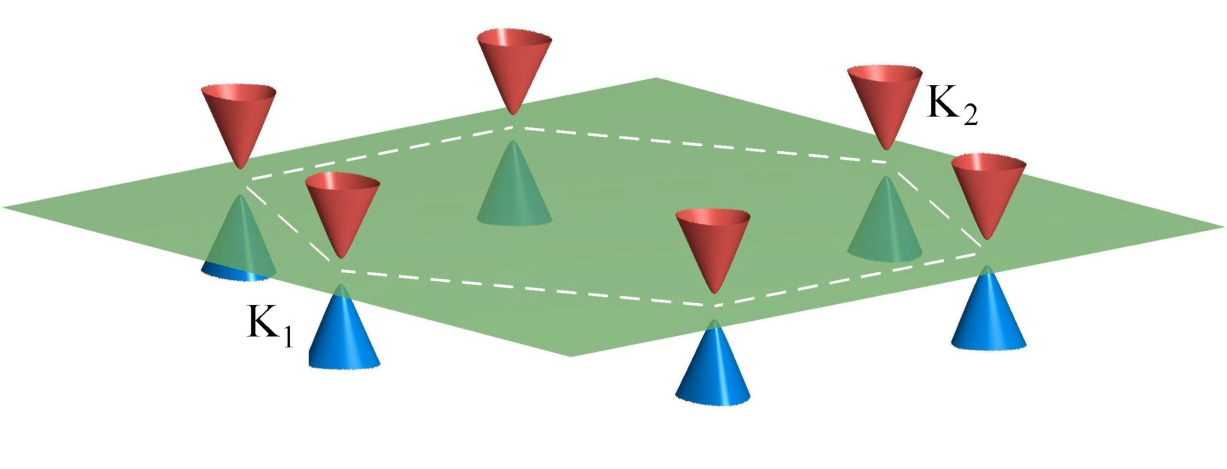
\includegraphics[width=0.7\linewidth]{Immagini/ValleyHall/band_graphene.pdf}
    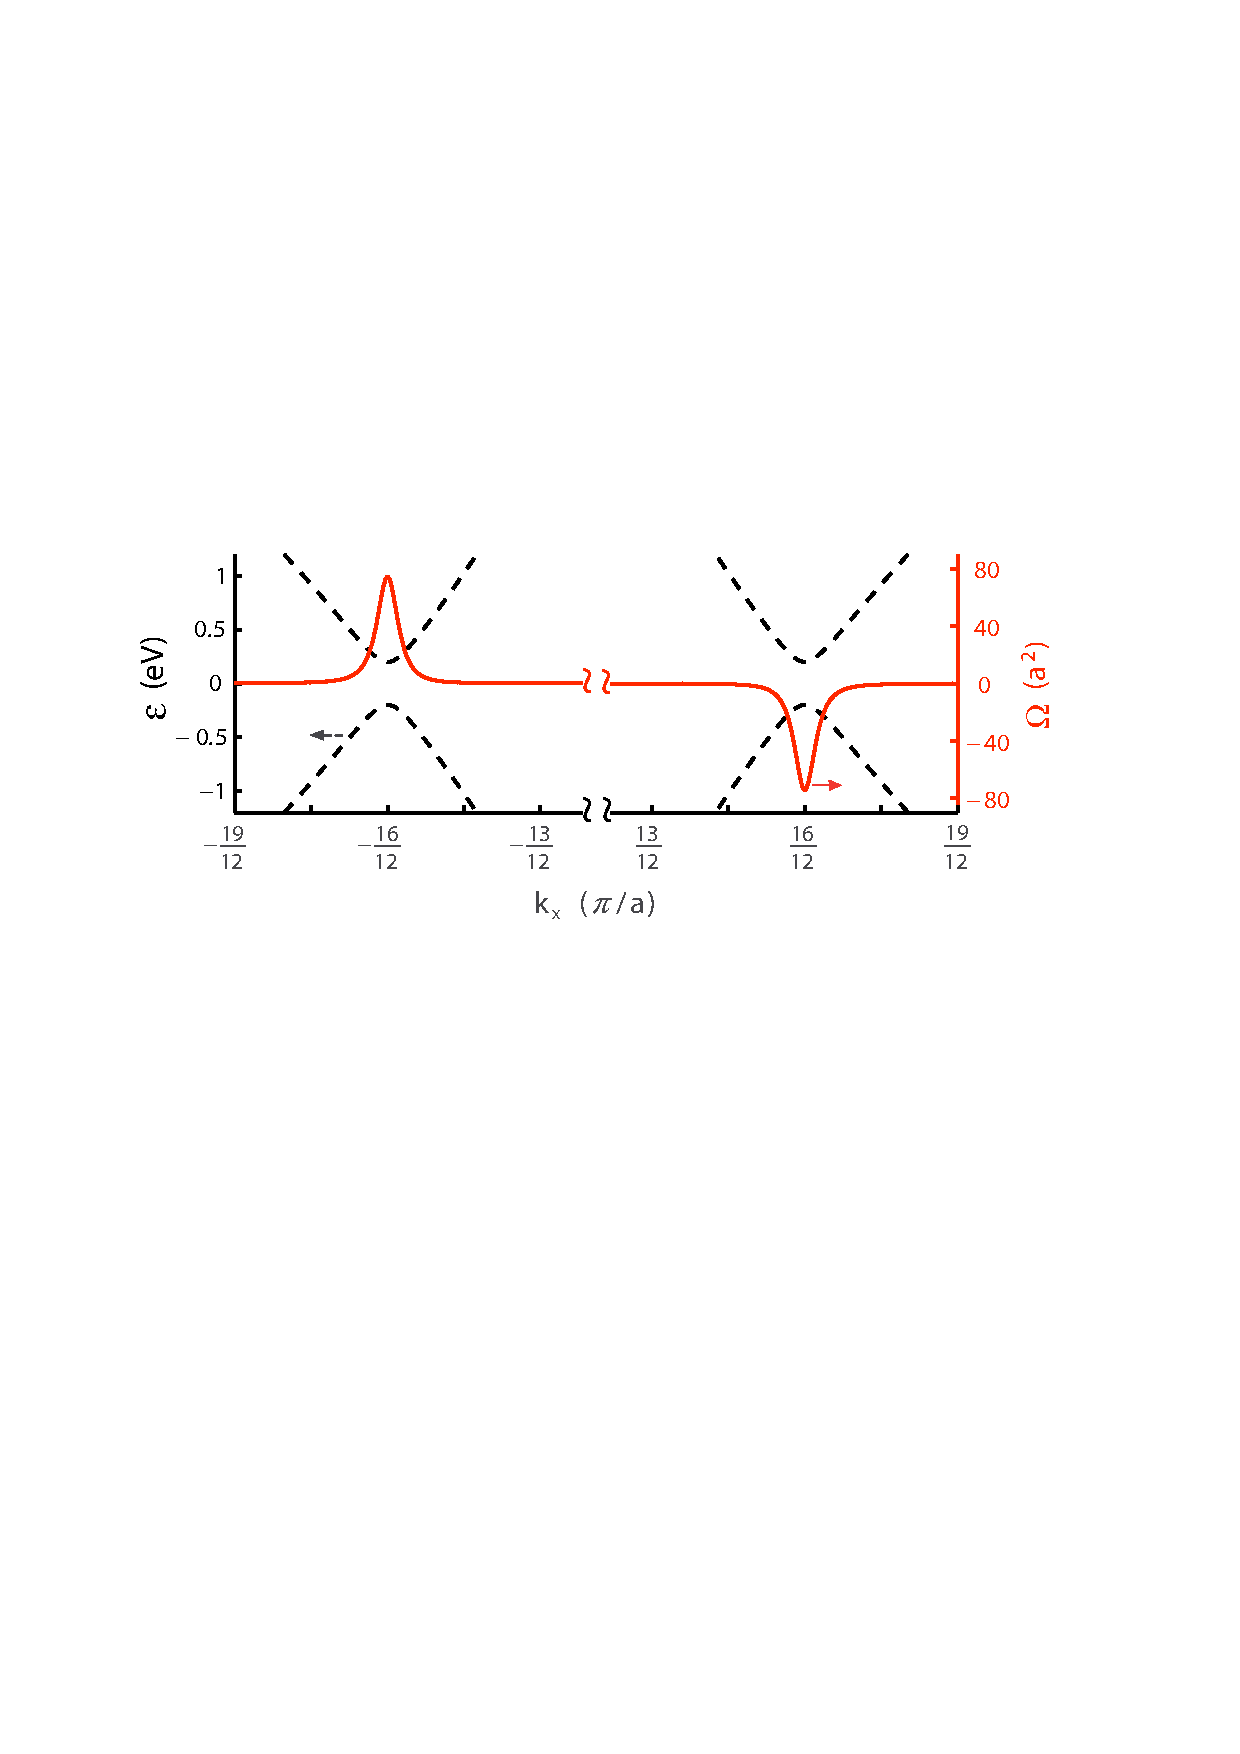
\includegraphics[width=0.7\linewidth]{Immagini/ValleyHall/curvature_graphene.pdf}
    \caption{In the top panel are displayed the Energy bands in 2D. In the bottom panel with the dotted line are displayed a section of the energy bands, and with the continuous red line the Berry curvature.}
    \label{fig:cones}
\end{figure}









 

\section{Valley-Hall effect}
The Hall conductivity $\sigma_{xy}$ is 
\begin{equation}
    \sigma_{xy}=\frac{e^2}\hbar \int_{\mathbb R^2} f[E^+(k)]\Omega^+_{k_xk_y}+f[E^-(k)]\Omega^-_{k_xk_y}\frac{d^2\vect k}{2\pi}
    \label{eq:valley-conductivity-1}
\end{equation}
Where $f(E)=\big[e^{\beta (E-\mu)}+1\big]^{-1}$ is the Fermi-Dirac distribution, it is applied once for the states with positive energy and once for the states with negative energy.

We are going to analyze the system at low temperatures ($k_bT\ll 1$), so our Fermi-Dirac distribution can be considered like a step-function.

First let's integrate the conductivity for the positive energies and drop the $+$ sign to make the notation lighter.

\[
    \int_{\mathbb R^2} f[E(k)]\Omega_{k_xk_y}dk_xdk_y=\int_{\mathbb R^2} f[E(q)]\Omega_{q_xq_y}dq_xdq_y\approx
\]

\[
    \approx\int_{0}^{2\pi}\int_{0}^{q_F}\frac12 \frac{\Delta^2}{q^2E^3}(q_x+q_y-2q)qdqd\theta=
\]

\[
    =-2\pi\Delta^2\int_0^{q_f}\frac{dq}{E^2} =-2\pi\Delta^2\int_0^{q_f}\frac{dq}{(\Delta^2+q^2)^{3/2}}= 
    -\frac{2\pi q_F}{\sqrt{\Delta^2+q_F^2}}
\]

And now we express it in terms of the chemical potential $\mu$ \footnote{Here we can use interchangeably $\mu$ and $E_F$}


\begin{equation}
    \int_{\mathbb R^2} f[E(k)]\Omega_{k_xk_y}dk_xdk_y\approx-2\pi \frac{\sqrt{\mu^2-\Delta^2}}\mu\theta(\mu-\Delta)
\end{equation}
The $\theta(\mu-\Delta)$ is there to make sure that if no states are inside the Fermi-Dirac the integral is zero. One thing to notice is that if you have $\mu \gg \Delta$ (aka. all states in the band are occupied) then the integral is equal to $-2\pi$. The integral of the lower band is very similar. By the end equation of the conductivity \ref{eq:valley-conductivity-1} becomes
\begin{equation}
    \sigma_{xy}(\mu)=-\frac {e^2}{2\pi \hbar}\Bigg[\frac{\sqrt{\mu^2-\Delta^2}}{\mu} \theta(\mu^2-\Delta^2) - \theta(\mu-\Delta)\Bigg]
    \label{eq:valley-conductivity-2}
\end{equation}
\begin{figure}
    \centering
    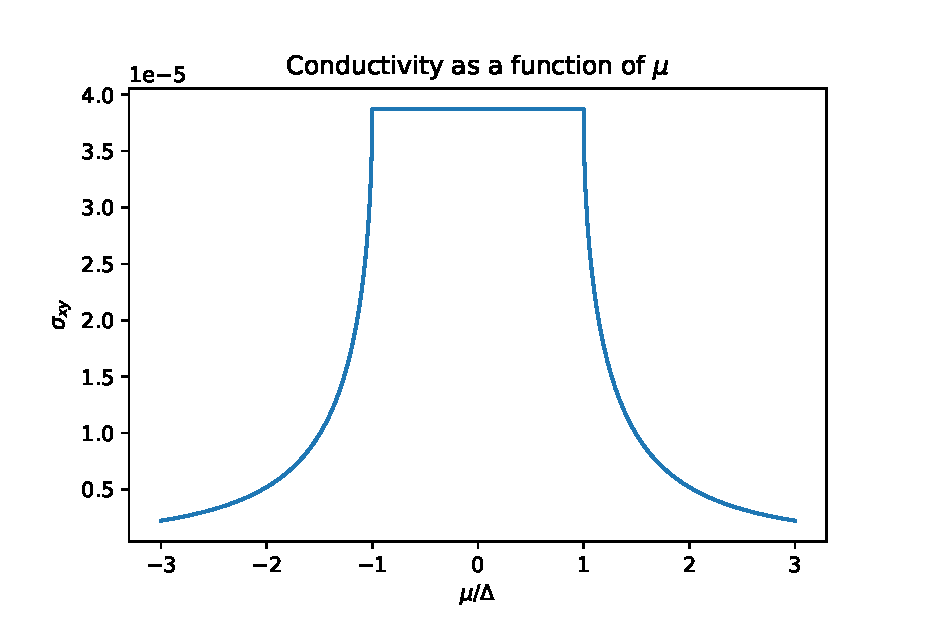
\includegraphics[width=\linewidth]{Immagini/ValleyHall/sigma_xy.eps}
    \caption{Here is shown $\sigma_{xy}(\mu)$ (eq. \ref{eq:valley-conductivity-2}). Notice how, when $\mu \in [-\Delta,\Delta]$ then $\sigma_{xy}=\frac {e^2}{2\pi \hbar}$}
    \label{fig:sigma_xy}
\end{figure}
To be fear we only calculated $\sigma_{xy}$ for the electrons in the valley $K_1$, the conductivity for the other valley is just $-\sigma_{xy}$. So, putting it all together, we have

\begin{equation}
    \sigma_{K_i,xy}(\mu)=(-1)^i\frac {e^2}{2\pi \hbar}\Bigg[\frac{\sqrt{\mu^2-\Delta^2}}{\mu} \theta(\mu^2-\Delta^2) - \theta(\mu-\Delta)\Bigg]
    \label{eq:valley-conductivity-complete}
\end{equation}
However in most cases it's safe to assume that the chemical potential is inside the energy gap, so equation \ref{eq:valley-conductivity-complete} becomes
\begin{equation}
    \sigma_{K_i,xy}=(-1)^{i+1}\frac {e^2}{2\pi \hbar}
\end{equation}



\section{Non-local Charge transport}
If we apply a voltage $V$ in two opposite points of a strip of a ohmic material of width $W$ and infinite lenght, and  we see a current that flows from one point to another figure \ref{fig:beconcini_strip}.\newline
\begin{figure}
    \centering
    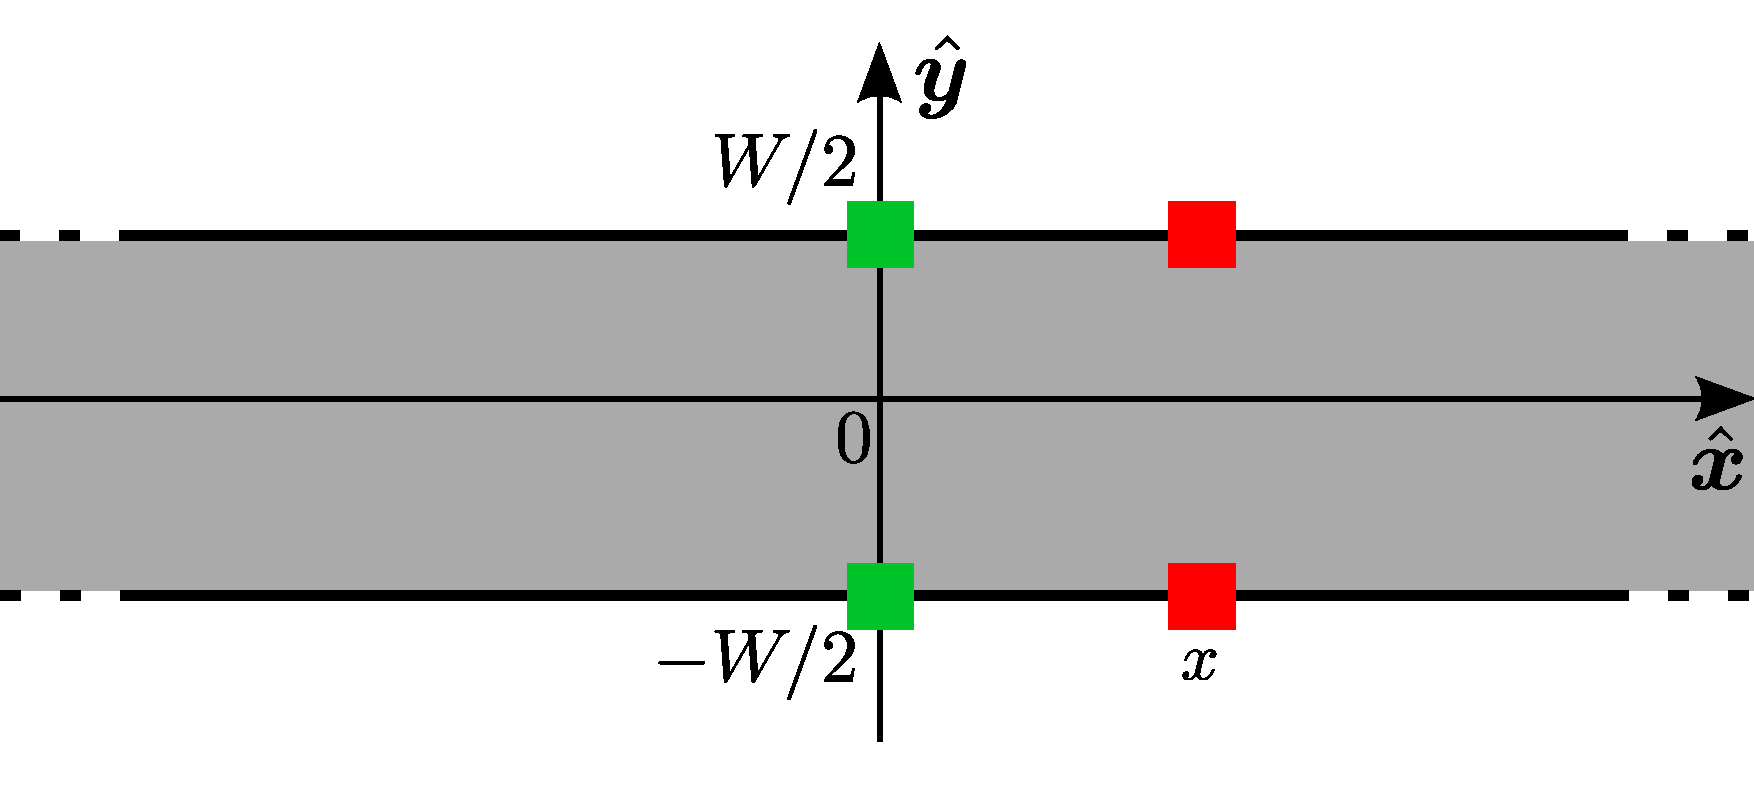
\includegraphics[width=0.7\linewidth]{Immagini/ValleyHall/beconcini_strip.pdf}
    \caption{Representation of the strip}
    \label{fig:beconcini_strip}
\end{figure}
Clearly the current isn't completely localized along the axis that unites the two injection points, and so does the voltage difference.\newline
If we probe the voltage from two different points with an offset of $x$ from the injection points and we divide it by the total current between the contacts we see that  

\begin{equation}
    \frac{V(x)}I=\frac{2\rho}\pi\ln\bigg |\coth \Big(\frac{\pi x}{2W}\Big)\bigg |
\end{equation}
Where $\rho$ is the resistivity. Don't worry later on there is the proof of this equation.\newline

However, two-dimentional material like gapped graphene \cite{gorbachev2014detecting,sui2015gate,shimazaki2015generation} and transition-metal dichalcogenides \cite{xiao2012coupled,mak2014valley,lee2017valley}, don't obey this equation.\newline
This is because theese materials display the Valley Hall effect we talked about previously (inserire reference a sezione).\newline
Non-local transport can be a useful tool to probe the existance of anomalous Hall effect \cite{valenzuela2006direct,abanin2009nonlocal,brune2010evidence,abanin2011giant,balakrishnan2013g,wang2015proximity}


\section{Theory of non local charge transport}

Let $K_1$ and $K_2$ be the two valleys in our honeycomb material (figure \ref{fig:cones}). Their Berry curvature is 




Each of the two cones will have an excess of density of electrons $n_K(\vect r)$ with $K\in \{K_1,K_2\}$
	\section{Study of $R_{NL}$}
Unfortunately \ref{eq:rnlk} doesn't have an analytic Fourier transform. If there are no topological effect, so $\tan (\theta_{VH})=0$, it can be solved analytically.

\begin{equation}
    R_{NL}(x)=\frac 2{\sigma_c}\int_{-\infty}^{+\infty}
    \frac{\tanh (kW/2)}k \frac {dk}{2\pi}=
    -\frac{2\rho}\pi\ln\bigg |\tanh \Big(\frac{\pi x}{2W}\Big)\bigg |
    \label{eq:ohmic signal2}
\end{equation}
This is the purely ohmic nonlocal signal that we have talked about in \ref{eq:ohmic signal}.

However if we are going to explore topological materials we cannot set $\tan (\theta_{VH})=0$, rhis means that we'll have to explore equation \ref{eq:rnlk} in regimes where it is approximately equal to a function that admits an analytic Fourier transform.

Let's look at the graph of the $R_{NL}(k)$ before doing any approximations:
\begin{figure}[h!]
    \centering
    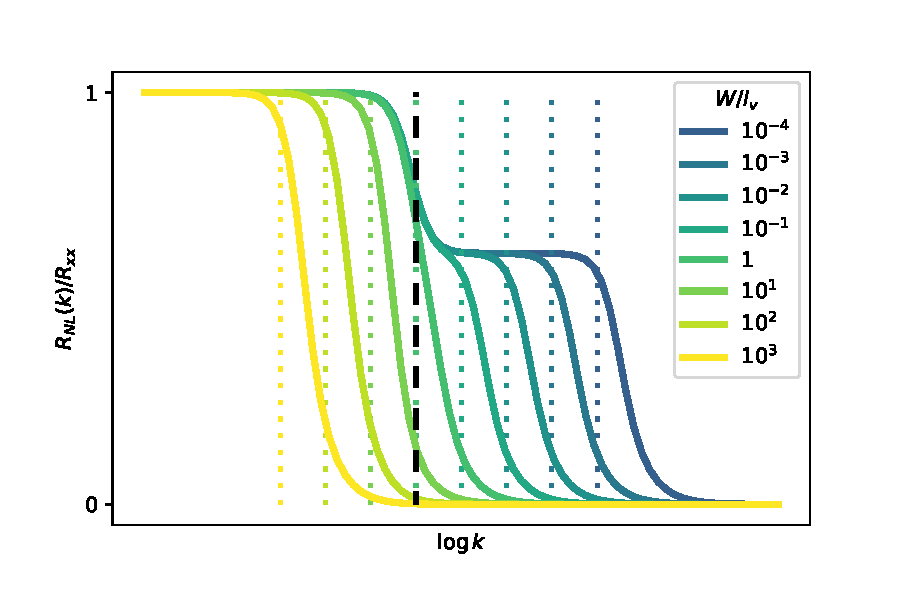
\includegraphics[width=\linewidth]{Immagini/rnl/widths.pdf}
    \caption{$R_{NK}(k)$ for several values of $W/l_v$. The dashed black line represents where $k=1/l_v$, the colored dashed line represents where $k=1/W$}
    \label{fig:RNLk}
\end{figure}
As you can see from the figure \ref{fig:RNLk} if $W\gg l_v$ we have a single bell like function with the width of the bell being $\approx 1/W$. If $W\ll l_v$ we have a double-bell function, where the first bell has a height of $1$ and a width of $1/l_v$, and the second one has a shorter height. To evaluate the precise height we just need to set $l_v^{-1}\ll k \ll W^{-1}$ in equation \ref{eq:rnlk}, this gives us 
,

\begin{equation}
    R_{NL}(l_v^{-1}\ll k \ll W^{-1})\approx \frac{R_{xx}}{1+\tan^2(\theta_{VH})}   
    \label{eq:plateau} 
\end{equation}
Where $R_{xx}=\frac{W}{\sigma_{xx}}$

So, if we have $l_v\ll W$ or $\tan(\theta_{VH})\ll 1$ (or both) we have a single bell structure. Incidentally these are the conditions to NOT have topological effects, so the less visible the double bell is, the less visible the topological effects are. We'll also see later how one of the bell represents the ohmic nonlocal signal, while the other represents the topological nonlocal signal. 


Let's start by exploring $k\ll l_v^{-1},W^{-1}$. This will tell us how the function behaves for $x\gg l_v,W$. In this regime 

\begin{equation}
    \omega(k)\approx \frac 1{l_v}\bigg[1+\frac{(kl_v)^2}2\bigg]\quad\quad
    \coth (kW/2)\approx \frac 2{kW} + \frac{kW}6
\end{equation}
Plugging this into equation \ref{eq:rnlk} we have that $R_{NL}(k)\approx$
\begin{equation}
    \frac 2{\sigma_c}\frac 1 {l_vk}\Bigg[
        \frac 1{l_v}\bigg(1+\frac{k^2l_v^2}{2}\bigg)\bigg(\frac 2{kW} + \frac{kW}6\bigg)+
        \frac{k\tan^2(\theta_{VH})}{\tanh(W/2l_v)} + o(k^2)
    \Bigg]^{-1}
\end{equation}
With some mathematical manipulation it can be shown that it is equal to 
\begin{equation}
    R_{NL}(k\ll l_v^{-1},W^{-1})=
    \frac W{\sigma_c}\frac 1{1+L_v^2k^2} + o(k^3)
    \label{eq:lorentz1}
\end{equation}
where the renormalized valley diffusion length $L_v^2$ is 
\begin{equation}
    L_v^2 = l_v^2+\frac {W^2}{12} +\frac{l_vW}2 \frac{\tan^2(\theta_{VH})}{\tanh(W/2l_v)}
\end{equation}
Now we do the Fourier transform of equation \ref{eq:lorentz1} ignoring the $o(k^3)$ term to get the behavior of $R_{NL}(x\gg l_v,W)$
\begin{equation}
    R_{NL}(x\gg l_v,W)=\mathcal F^{-1}R_{NL}(k\ll l_v^{-1},W^{-1}) 
    \label{eq:rxg}
\end{equation}
That is equal to 

\begin{equation}
    \frac W{\sigma_c}\int_{-\infty}^{+\infty}
    \frac 1{1+L_v^2k^2}
    \frac {dk}{2\pi}=
    \frac{W\rho}{2L_v}e^{-\frac{|x|}{L_v}}
\end{equation}
So,
\begin{equation}
    R_{NL}(x\gg l_v,W)=\frac{W\rho}{2L_v}e^{-\frac{|x|}{L_v}}
    \label{eq:rxl}
\end{equation}


Now we are going to study what happens for $k\gg l_v^{-1}$, in this case $\omega(k) \approx k$, So

\begin{equation}
    R_{NL}(k\gg l_v^{-1})=\frac 2{\sigma_c}\frac{\tanh}k\bigg(\frac{kW}2\bigg)\frac 1{1+\tan^2(\theta_{VH})}
\end{equation}
it's Fourier transform is
\begin{equation}
    R_{NL}(x\ll l_v)=-\frac 2{\pi\sigma_c}\frac 1{1+\tan^2(\theta_{VH})} \ln\bigg |\tanh \Big(\frac{\pi x}{2W}\Big)\bigg |
\end{equation}
This last equation is $1+\tan^2(\theta_{VH})$ smaller to the one for the purely ohmic nonlocal signal (eq. \ref{eq:ohmic signal2})

Now let's see how these equations fear in practice
\begin{figure}[h!]
    \centering
    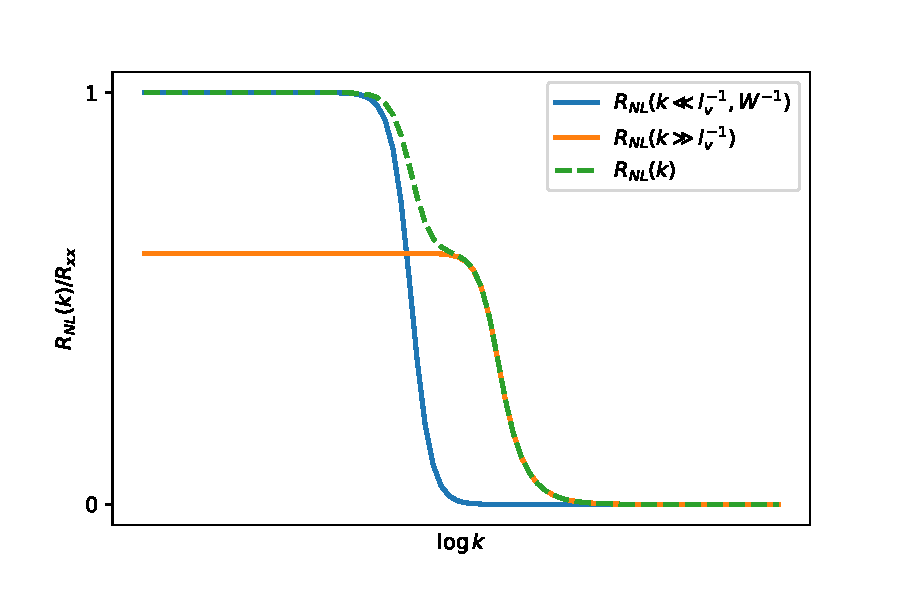
\includegraphics[width=\linewidth]{Immagini/rnl/2approx.pdf}
    \caption{For this example $l_v=20W$}
    \label{fig:rnl2approx}
\end{figure}
As you can see from figure \ref{fig:rnl2approx} the two approximations work pretty well, except in the neighborhood where $k\approx l_v^{-1}$. But what we really care about is $R_{NL}(x)$.\\
If we plot $R_{NL}(x\gg l_v,W)$ (eq. \ref{eq:rxg}) and $R_{NL}(x\ll l_v)$ (eq. \ref{eq:rxl}) alongside the numerical Fourier transform of $R_{NL}(k)$ \ref{eq:rnlk} we get figure \ref{fig:rnlx2approx}

\begin{figure}[h!]
    \centering
    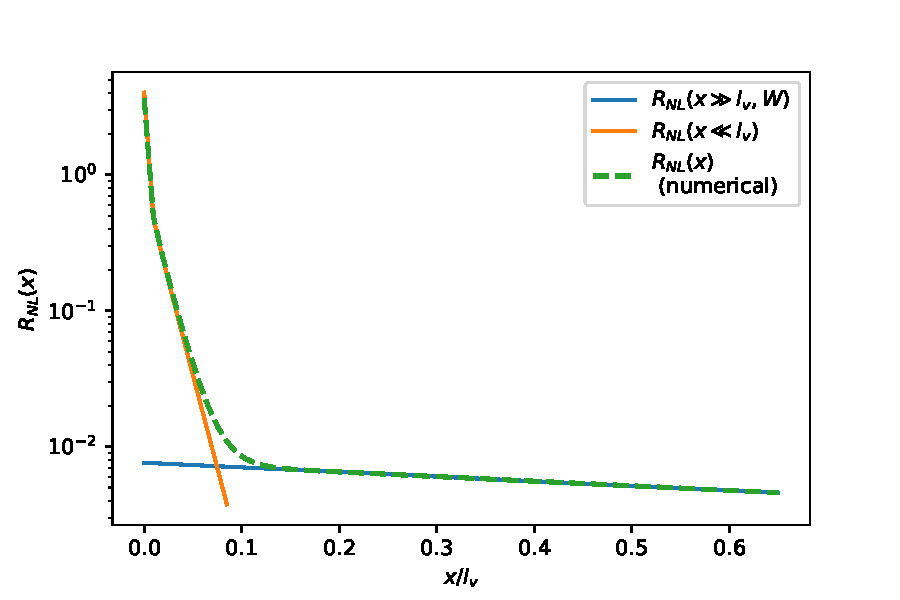
\includegraphics[width=\linewidth]{Immagini/rnl/x2approx.pdf}
    \caption{The parameters for this graph are exactly the same for the previous graph (figure \ref{fig:rnl2approx})}
    \label{fig:rnlx2approx}
\end{figure}
\subsection{Improving the approximation}
We can do better than this! By combining the two approximations it's possible to have a single equation that is very accurate for $k$ far from $l_v^{-1}$ ($(k-l_v^{-1})^2\gg 1$), but it ends up being reasonably good for $k\approx l_v^{-1}$ as well.\\
Since the Fourier transform is linear, the idea is to find the linear combination of the two approximation that best approximates the $R_{NL}(k)$.
\[
    R_{NL}(k)\approx \alpha R_{NL}(k\ll l_v^{-1},W^{-1}) +\beta R_{NL}(k\gg l_v^{-1})
\]
Where $\alpha$ and $\beta$ are the coefficient to be determined.\\
Since we only need to evaluate two variables, we only need to evaluate the expression above in two different points. The most reasonable points to choose are $k=0$ and $k=+\infty$, since they are the points where the approximations work better. For doing the calculations it's best to write out the two approximations 
\[
    R_{NL}(k)\approx 
    \alpha \frac W{\sigma_c}\frac 1{1+L_v^2k^2}+
    \beta\frac 2{\sigma_c}\frac{\tanh}k\bigg(\frac{kW}2\bigg)\frac 1{1+\tan^2(\theta_{VH})}
\]
The term that is multiplied by $\beta$ for $k\to +\infty$ is an increasingly precise estimate of $R_{NL}(k)$, and it dominates over the term that is multiplied by alpha, so $\beta=1$.\\
If we set $k=0$ we have that
\[
    R_{xx}=\alpha R_{xx} +  \frac {R_{xx}}{1+\tan^2(\theta_{VH})}   
\]
So, $\alpha=\big[1+\tan^{-2}(\theta_{VH})\big]^{-1}$. Putting it all together we define the resulting approximation
\begin{equation}
    \boxed{
        \tilde R_{NL}(k)\equiv
        \frac {R_{xx}}{1+L_v^2k^2}\frac 1{1+\tan^{-2}(\theta_{VH})}+
        \frac 2{\sigma_c}\frac{\tanh}k\bigg(\frac{kW}2\bigg)\frac 1{1+\tan^2(\theta_{VH})}
    }
\end{equation}
And if we plot the approximation $\tilde R_{NL}(k)$ alongside the actual values of $R_{NL}(k)$ we can see that they are remarkably similar (figure \ref{fig:kapproxcomp})
\begin{figure}[h!]
    \centering
    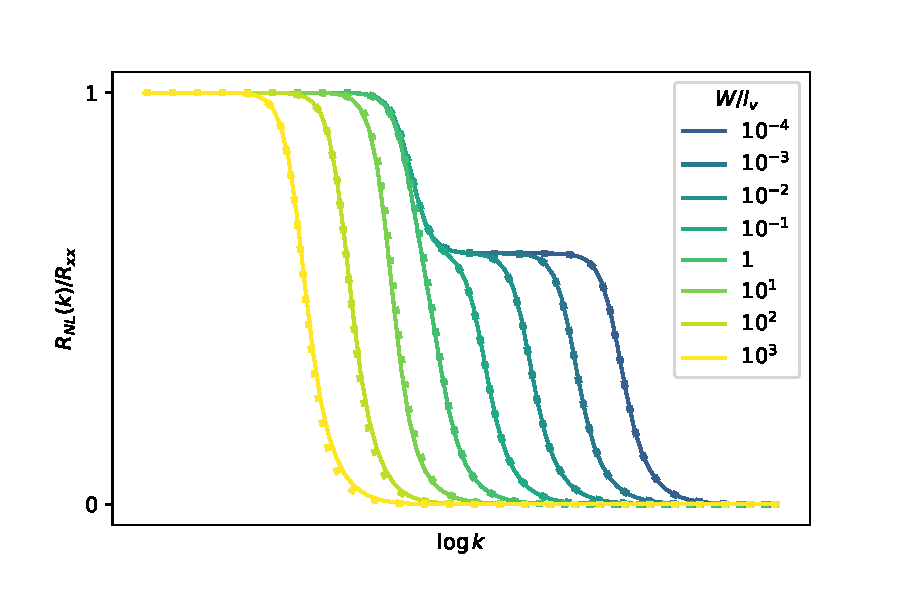
\includegraphics[width=\linewidth]{Immagini/rnl/kapproxcomp.pdf}
    \caption{Comparison between $R_{NL}(k)$ and $\tilde R_{NL}(k)$. The continuous line represents $R_{NL}(k)$, while the dashed line represents $\tilde R_{NL}(k)$}
    \label{fig:kapproxcomp}
\end{figure}\\
The nice thing about this is that if two equations are similar, then their Fourier transform will be too. We can transform $\tilde R_{NL}(k)$ with equations \ref{eq:rxg} and \ref{eq:rxl} and we get that

\begin{equation}
    \boxed{
        \tilde R_{NL}(x)=
        \frac{W \rho_{c,xx}e^{-|x|/L_v}}{2L_v[1+\tan^{-2}(\Theta_{VH})]}-
        \frac{2\rho_{c,xx}}{\pi [1+\tan^2(\Theta_{VH})]}\ln \bigg|\tanh \Big(\frac{\pi x}{2W}\Big)\bigg|
    }
\end{equation}
Infact if we re-create figure \ref{fig:rnlx2approx} with the equation above we get figure \ref{fig:rnlxapprox}
\begin{figure}[h!]
    \centering
    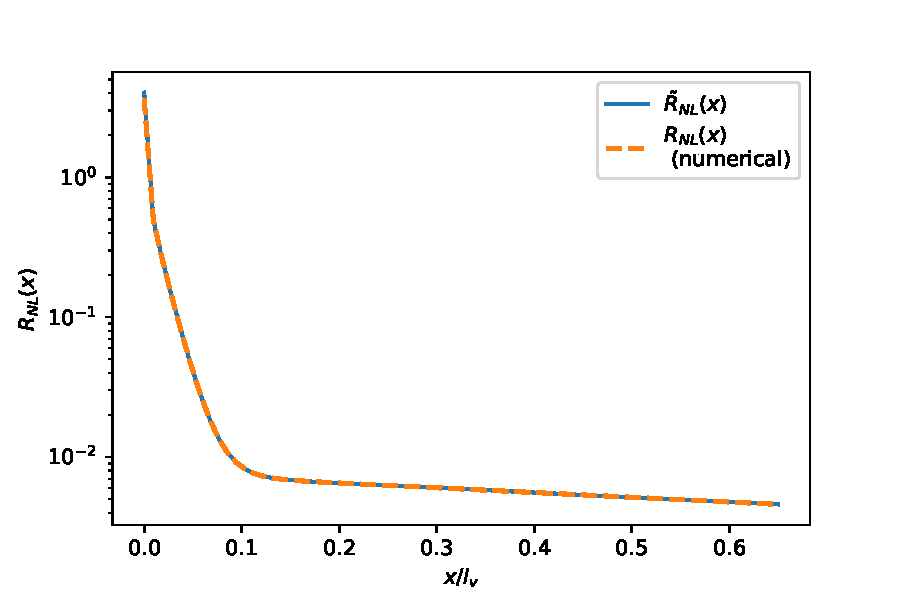
\includegraphics[width=\linewidth]{Immagini/rnl/xapprox.pdf}
    \caption{As you can see it's impossible to distinguish the difference between the two functions to the naked eye. The parameters are the same as figure \ref{fig:rnlxapprox}}
    \label{fig:rnlxapprox}
\end{figure}
	\section{$R_{NL}(x)$ as we change $\rho_{xx}$}
Hall effect experiments are generally done in the so-called Hall-bars. There are samples of material with a shape like the one in figure \ref{fig:hall-bar}. This also means that more often than not in experimental setups we cannot change $x$ without changing the geometry of the sample.
\begin{figure}[h!]
    \centering
    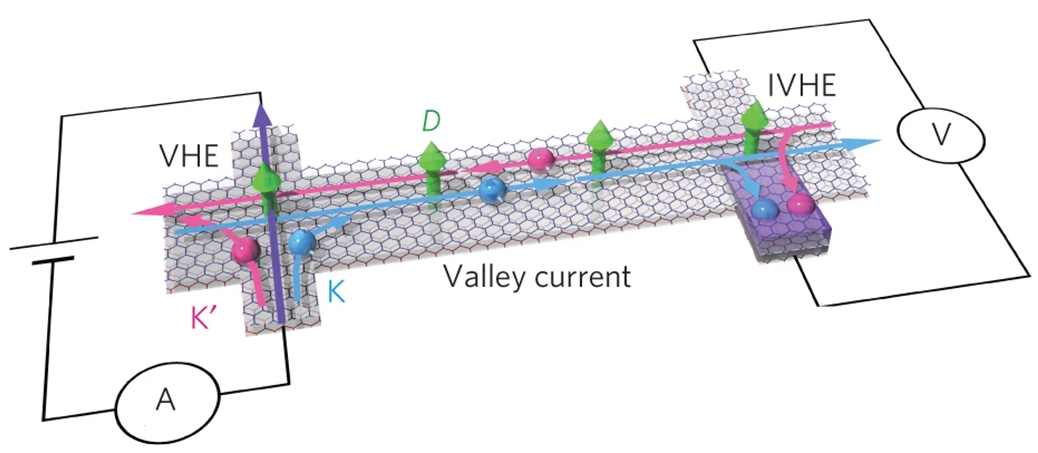
\includegraphics[width=\linewidth]{Immagini/rnl/hallbarbrutta.png}
    \caption{Example of the experimental setup}
    \label{fig:hall-bar}
\end{figure}\\
In the previous section we studied how $R_{NL}$ depended on $x$, and Hall-bars can only measure a single $x$. One way for having multiple measuraments with the same Hall-bar is to change the resistivity of the material by changing the temperature of the setup, and study $R_{NL}$ as we change $\rho_{xx}$.

For convenience let's re-write equation \ref{eq:rnlk}
\[
    R_{NL}(k)=\frac{2\omega(k)}{k\sigma_c}
    \bigg\{
        \frac{\omega(k)}{\tanh(kW/2)} + \frac{k\tan^2(\theta_{VH})}{\tanh[\omega(k)W/2]}    
    \bigg\}^{-1}
\]
For convenience, we are going to change $\tan(\theta_{VH})=\sigma_v\rho_{xx}$ and do a taylor series expansion of the above equation around $\tan^2(\theta_{VH})\approx 0$.

\[
    R_{NL}(k)\approx R_{NL}(k)|_{\tan^2(\theta_{VH})=0} +
    \frac \partial {\partial \tan^2(\theta_{VH})} R_{NL}(k)|_{\tan^2(\theta_{VH})=0}
\]
that we are going to re-define as
\[
    R_{NL}(k)\approx R_{NL}^{(0)}(k) + R_{NL}^{(1)}(k)
\]
The zeroth order term gives us this:
\[
    R_{NL}^{(0)}(k)=\frac{2\rho}k\tanh\bigg(\frac{kW}2\bigg)
\]
And if we do a the Fourier transform to get the $x$ dependent form we get the ohmic nonlocal resistivity \ref{eq:ohmic signal}
\begin{equation}
    R_{NL}^{(0)}(x)=\frac{2\rho}\pi\ln\bigg |\coth \Big(\frac{\pi x}{2W}\Big)\bigg |
\end{equation}
Now let's calculate the first order term

\[
    R_{NL}^{(1)}(k)=-2\rho\frac{\omega(k)}k\bigg[\frac{\omega(k)}{\tanh(Wk/2)} \bigg]^{-2}k\frac{\tan^2(\theta_{VH})}{\tanh(\omega(k)W/2)}=
\]
\[
    =-2\rho^3\sigma_v^2 \tanh^2\bigg(\frac{kW}2\bigg)\bigg\{\omega(k)\tanh\bigg[\frac{\omega(k) W}2\bigg]\bigg\}^{-1}\equiv
    \rho^3F(k)
\]
where $F(k)$ is defined as follows

\begin{equation}
    F(k)\equiv -2\sigma_v^2\tanh^2\bigg(\frac{kW}2\bigg)\bigg\{\omega(k)\tanh\bigg[\frac{\omega(k) W}2\bigg]\bigg\}^{-1}
\end{equation}
And it doesn't depend on $\rho$

Putting it all together we get that

\begin{equation}
    \lim_{\rho\to 0} R_{NL}(x)= \frac{2\rho}\pi\ln\bigg |\coth \Big(\frac{\pi x}{2W}\Big)\bigg | + \rho^3F(x) + o(\rho^5)
\end{equation}

PARLARE DEI REGIMI IN CUI DOMINA $\rho^3$

Now let's study what happens when $\rho,\tan(\theta_{VH})\to \infty$. First off let's rewrite equation \ref{eq:rnlk} and bring the $\omega(k)$ and $k$ inside the curly braces.

\[
    R_{NL}(k)=2\rho
    \bigg\{
        \underbrace{\frac{k}{\tanh(kW/2)}}_{\substack{\text{cannot be}\\\text{ignored for } k=0}} + \frac {k^2}{\omega(k)}\frac{\tan^2(\theta_{VH})}{\tanh[\omega(k)W/2]}    
    \bigg\}^{-1}
\]

This limit is a bit tricky to evaluate. First off even thought the right-most term inside the curly braces dominates everywhere except for $k=0$ this "\emph{small detail}" is crucial. From image \ref{fig:rho1} we can see that the larger $\rho$ gets, the smaller the area around $k=0$ where the first term dominates.
\begin{figure}[h!]
    \centering
    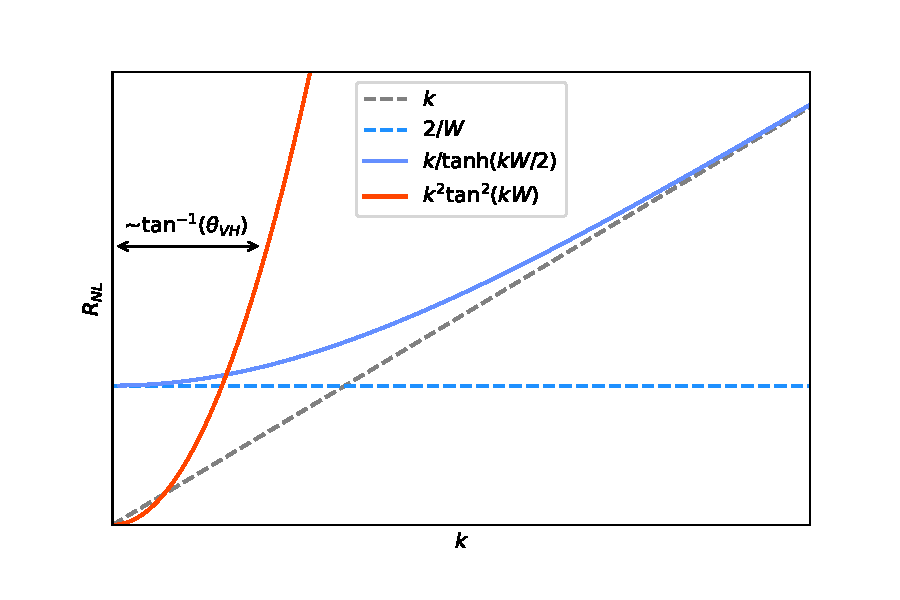
\includegraphics[width=\linewidth]{Immagini/rnl/rho1.pdf}
    \caption{The continuous blue line represents the first term, the blue dashed line represents its approximation around $k=0$ and the gray dashed lines represent its approximation for $k\to \infty$.\newline The orange parabola represents the right-hand side term $\frac {k^2}{\omega(k)}\frac{\tan^2(\theta_{VH})}{\tanh[\omega(k)W/2]}$}
    \label{fig:rho1}
\end{figure}\\
For high values of $\rho, \tan(\theta_{VH})$ the parabola becomes really narrow and it overtakes the first term with $k\approx 0$. This means that we can approximate the first term as being always equal to $2/W$. This means that
\begin{equation}
    \lim_{\rho\to\infty} R_{NL}(k)=2\rho
    \bigg\{
        \frac 2W+ \frac {k^2}{\omega(k)}\frac{\tan^2(\theta_{VH})}{\tanh[\omega(k)W/2]}    
    \bigg\}^{-1}
\end{equation}



	\section{Comparison with experimental data}
Experimental setups have a few limitations compared to the theoretical treatment, for example you don't have complete freedom of changing the resistance, rather the resistance is changed by changing the temperature of the sample.
This has a few consequences: 
\begin{itemize}
    \item Since out sample is a semiconductor, the lower the temperature, the higher the resistance, but if the temperature gets too low we enter the ballistic regime, and our treatment is no longer valid.
    \item If the temperature gets too high, the quantization of the hall effect disappears
\end{itemize}
This restricts us to a couple order of magnitude of the resistivity.

Now we compare the results with the experimental data. Let's start from analyzing the data from  \cite{rebecca2022moirè}.\\
In this paper the authors measured the valley hall effect of a heterostructure made of bilayer-graphene on top of boron nitride at different angles $\phi$ between the graphene and the boron nitride. The sample has a width $W=1.7\mu$m, and inter-valley scattering length $l_{\textrm v}=1.6\mu$m and the distance of the contact from the injection point is $x=2.3\mu$m

The angles $\phi$ that were explored are $0,\pi/6$ and $\pi/3$. If you plot the measurements you get figure \ref{fig:rebeccadatapoints}

\begin{figure}[h!]
    \centering
    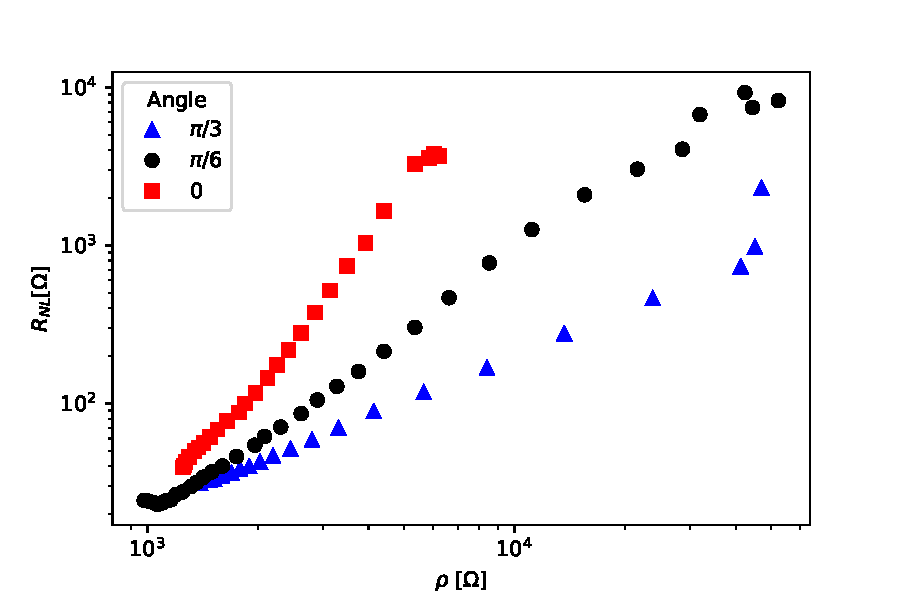
\includegraphics[width=\linewidth]{Immagini/rnl/rebecca_data.pdf}
    \caption{Datapoints from \cite{rebecca2022moirè}}
    \label{fig:rebeccadatapoints}
\end{figure}

Now we analyze them one by one
\begin{itemize}
    \item For $\phi=\pi/3$ we have that the response is fully ohmic, and so we get a completely linear response (figure \ref{fig:rebecca pi/3})
    \item For $\phi=\pi/6$ we have a hall effect, however, since $W\approx l_\textrm{v}$ the ohmic and the topological response mix together, so we never see the full-fledged $\rho^3$ behavior.\footnote{A more detailed explanation was given in the details of subsection \ref{sec:alternaterho}}
\end{itemize}
\begin{figure}[h!]
    \centering
    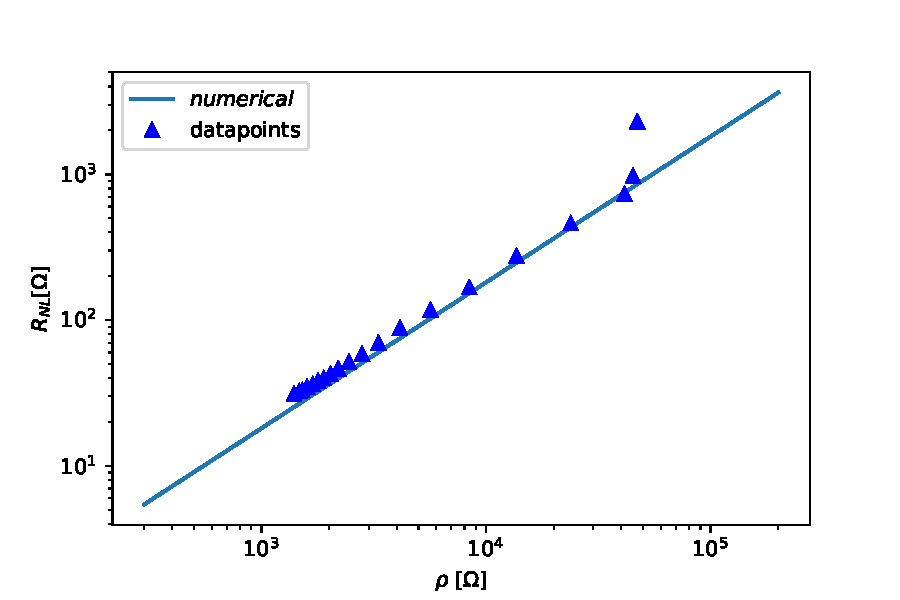
\includegraphics[width=\linewidth]{Immagini/rnl/rebecca_0.pdf}
    \caption{Comparison between the data points and the theoretical expectation for $\phi=\pi/3$. The last point is an outlier, but all in all it looks pretty good}
    \label{fig:rebecca pi/3}
\end{figure}


\begin{figure}[h!]
    \centering
    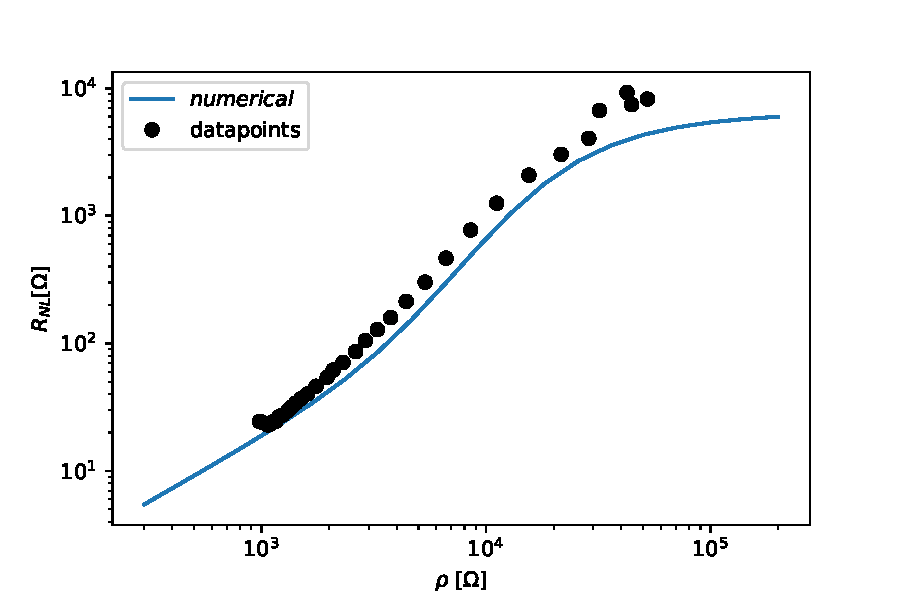
\includegraphics[width=\linewidth]{Immagini/rnl/rebecca_1.pdf}
    \caption{Comparison between the data points and the theoretical expectation for $\phi=\pi/6$. The model has a lower precision for higher values of $\rho,R_{\textrm{NL}}$}
    \label{fig:rebecca pi/6}
\end{figure}
	\section{Berry phase}
    Berry phase is the simplest demonstration of how geometry and topology can emerge from quantum mechanics and it is at heart of the quantum Hall effect.\newline
    Let us consider a physical system described by a Hamiltonian that depends on a set of parameters $\boldsymbol \lambda=(\lambda_1,\lambda_2,\dots)$. These parameters do not represent the degrees of freedom of the system like position and momentum, rather they describe things such as the mass of a particle, the strength of a potential and so on.\\ For each $H(\boldsymbol \lambda)$ there exists a set of eigenstates such that 
    \begin{equation}
        H(\boldsymbol \lambda)\ket{n,\boldsymbol \lambda}=E_n(\boldsymbol \lambda)\ket{n,\boldsymbol \lambda}\,,
    \end{equation}
    however the equation above does not completely determine the basis function $\ket{n,\boldsymbol \lambda}$; We can change arbitrarily the phase $\gamma_n(\boldsymbol \lambda)$ of any eigenstate which is called \textbf{Berry phase}
    \begin{equation}
        \label{eq:berryphase}
        \ket{n,\boldsymbol \lambda}\to \underbrace{e^{i\gamma_n(\boldsymbol \lambda)}}_{\textrm{Berry phase}} \ket{n,\boldsymbol \lambda}\,.  
    \end{equation}
    Suppose we start off with a Hamiltonian and then we slowly change the parameters for a time $T$ until it reaches a different Hamiltonian, this means that $\boldsymbol \lambda=\boldsymbol \lambda(t)$. For the adiabatic theorem we can say that if we start on an energy eigenstate, and the system changes slowly enough,and has no degeneracies, then the system will cling on that energy eigenstate.How slow you have to be in changing the parameters depends on the energy gap from the state you're in to the nearest other state. The smaller the gap, the slower you have to change the parameters. A way of showing this without doing long calculations is the following: \\ We know from the Heisenberg uncertainty principle that $T \Delta E \ge \hbar/2$. We want the uncertainty in the Energy to be way smaller than the energy gap $E_g \gg\Delta E$, so $E_g \gg \frac{\hbar}{2T}$, therefore if we make $T$ big enough it can be achieved.
    
    The equation of motion of a particle that for time $t=0$ is equal to $\ket{\psi_n(t=0)}=\ket{n,\boldsymbol \lambda(0)}$ is 
    \begin{equation}
        \label{eq:psin}
        |\psi_n(t)\rangle=\underbrace{e^{i\gamma_n(\boldsymbol \lambda (t))}}_{\textrm{Berry phase}}\cdot
        \underbrace{e^{-\frac i\hbar\int_0^t E_n(\boldsymbol \lambda (t')) dt'}}_\textrm{dynamical phase}|n,\boldsymbol \lambda (t)\rangle  \,,    
    \end{equation}
    where the first exponent comes from eq. \ref{eq:berryphase}. We now insert the equation above into the time-dependent Schrodinger equation
    \begin{equation}
        \label{eq:shrodt}
        i\hbar\partial_t|\psi_n(t)\rangle=H(\boldsymbol \lambda(t)) |\psi_n(t)\rangle\,.
    \end{equation}
    By plugging equation \ref{eq:psin} into the \textit{right} term term of equation \ref{eq:shrodt} we get we get that
    \begin{equation}
        \label{eq:H(t)}
        H(\boldsymbol \lambda(t)) |\psi_n(t)\rangle = E_n(t)\ket{\psi_n(t)}\,,
    \end{equation}
    and by plugging equation \ref{eq:psin} into the \textit{left} term term of equation \ref{eq:shrodt} we get we get that

    \begin{equation}
        \label{eq:psin-t}
        i\hbar\partial_t|\psi_n(t)\rangle=
        -\hbar \dot \gamma_n(t)|\psi_n(t)\rangle + E_n(t)|\psi_n(t)\rangle + e^{i\phi_n(t)}\partial_t|n,t\rangle\,,
    \end{equation}
    where we have defined $e^{i\phi_n(t)} \equiv e^{i\gamma_n(\boldsymbol \lambda (t))}e^{-\frac i\hbar\int_0^t E_n(\boldsymbol \lambda (t')) dt'}$.

    By equating the right terms in equations \ref{eq:H(t)} and \ref{eq:psin-t} we get that 
    \begin{equation}
        \label{eq:psin-t-H}
            i\hbar e^{i\phi_nt(t)}\partial_t|n,t\rangle=\hbar\dot \gamma_n(t)\ket{\psi_n(t)} =\hbar\dot \gamma_n(t)e^{i\phi_n(t)}\ket{n,t}
    \end{equation}    
    now we multiply the term on the left and on the right of equation \ref{eq:psin-t-H} by $\hbar^{-1}e^{-i\phi_n(t)} \bra{n,t}$
    \begin{equation}
        \label{eq:psin-t-H-bra}
            \dot \gamma_n(t)=i\bra{n,t} \partial_t\ket{n,t}
    \end{equation}
    We can re-express it in terms of $\boldsymbol \lambda$
    \begin{equation}
        \label{eq:connection}
            \dot \gamma_n(t)=\dot{\boldsymbol \lambda}\cdot\underbrace{i\bra{n,t} \partial_{\boldsymbol \lambda}\ket{n,t}}_{\equiv \mathbf A_n(\boldsymbol \lambda)}\,,
    \end{equation}
    where
    \begin{equation}
        \vect A_n(\vect \lambda)=
        i\bra{n,t} \partial_{\boldsymbol \lambda}\ket{n,t}\,.
        \label{eq:berryconnection}
    \end{equation}
    $\mathbf A_n(\boldsymbol \lambda)$ called the \textbf{Berry connection}
    This means that we can calculate the total change in $\gamma_n(t)$ can be obtained by doing a line integral in the space of parameters $\boldsymbol \lambda$ over the path $\mathcal P$ of values that $\boldsymbol \lambda$ assumes during the time evolution

    \begin{equation}
        \label{eq:line_int1}
            \gamma_n=\int_\mathcal{P} \mathbf A_n(\boldsymbol \lambda) \cdot d\boldsymbol \lambda\,,
    \end{equation}


    \begin{equation}
        \label{eq:re-define}
        \ket{n,\boldsymbol \lambda}\to e^{if_n(\boldsymbol \lambda)}\ket{n,\boldsymbol \lambda}\,.
    \end{equation}
    Keep in mind however that the eigenstates are defined up to a phase, meaning that we can re-define the base vectors like so 
    (equation \ref{eq:re-define}). If we apply this substitution into the formula of $\mathbf A_n$ we have that

    \[
    \mathbf A_n(\boldsymbol \lambda) =i\bra{n,t} \partial_{\boldsymbol \lambda}\ket{n,t}\to i\bra{n,t} \partial_{\boldsymbol \lambda}\ket{n,t} - \partial_{\boldsymbol \lambda}f_n(\boldsymbol \lambda)\,,
    \]

    \begin{equation}
        \label{eq:gauge1}
        \mathbf A_n \to \mathbf A_n - \partial_{\boldsymbol \lambda}f_n\,.
    \end{equation}
        So the system is invariant under the gauge transformation in equation \ref{eq:gauge1}. If we do this transformation to equation \ref{eq:line_int1} we have that

    \[
        \gamma_n=\int_\mathcal{P} \mathbf A_n(\boldsymbol \lambda) \cdot d\boldsymbol \lambda - \int_\mathcal{P} \partial_{\boldsymbol \lambda}f_n(\boldsymbol \lambda) \cdot d\boldsymbol \lambda= \int_\mathcal{P} \mathbf A_n(\boldsymbol \lambda) \cdot d\boldsymbol \lambda + f(\boldsymbol \lambda(0))-f(\boldsymbol \lambda (T))\,.
    \]
    This means that if the path $\mathcal{P}$ is open we can always choose a function $f_n$ such that 
    $f(\boldsymbol \lambda(0))-f(\boldsymbol \lambda(T))=\int_\mathcal{P} \mathbf A_n(\boldsymbol \lambda) \cdot d\boldsymbol \lambda$, 
    thus we can conclude that one can always choose a suitable $f(\boldsymbol \lambda)$ such that $\gamma_n$ accumulated along the path $\mathcal P$ is calceled out leaving equation 
    \ref{eq:psin} with only the dynamical phase. 
    However if the path is closed $\boldsymbol \lambda(0)=\boldsymbol \lambda(T)$, in order to make the phase change
    in equation \ref{eq:re-define} single valued we must have that
    \[
    e^{f(\boldsymbol \lambda(0))-f(\boldsymbol \lambda(T))}=1\,,
    \]
    so 
    \[
        f(\boldsymbol \lambda(0))-f(\boldsymbol \lambda(T))=2n\pi \quad n\in \mathbb{Z}\,.
    \]
    This leads us to the important result that
    \begin{equation}
        \label{eq:closed-berry}
        \gamma_n=\oint_{\mathcal P} \mathbf A_n(\boldsymbol \lambda)\cdot d\boldsymbol \lambda + 2n\pi\,.
    \end{equation}
    This time, if the line integral is not a multiple of $2\pi$ (and there is no reason why it should) there is no way of choosing a suitable $f_n$ to
    cancel it out and the Berry phase in equation \ref{eq:psin} is there to stay



\section{Berry curvature}
    You might have noticed that equation \ref{eq:gauge1} is analogous to what happens in Electromagnetism with the vector potential. This means that we can try using the same mathematics and see where it leads us. However, in classic and relativistic electromagnetism $\dim(\vect A_\mu)$ is equal to respectively 3 and 4, in the case of the Berry curvature it can have any integer value.

    In EM from the gauge-dependent $\vect A$ are defined the gauge-indipendent field as follows:
    \begin{enumerate}
        \item in $3$D the magnetic field is defined as follows $B_i=\epsilon_{ijk} \partial_j A_k$
        \item in $(3+1)$D the Field tensor is defined as $F_{\mu\nu}=\partial_\mu A_\nu-\partial_\nu A_\mu$
    \end{enumerate}
    In both cases the resulting field is asymmetric under the exchange of the indices of the derivative and the indices of the vector potential. This requirement is what makes the resulting field gauge independent.
    
    With the same logic we can define a gauge field tensor derived from the Berry connection:
    \begin{equation}
        \label{eq:berry-curvature1}
        \boxed{
            \Omega_{\mu\nu}^n =\partial_\mu A^n_\nu(\boldsymbol \lambda) - \partial_\nu A^n_\mu(\boldsymbol \lambda)\,.
        }
    \end{equation}
    This new field tensor is defined as \textbf{Berry curvature}, and it is gauge independent just like 
    $\vect B$ and $F_{\mu\nu}$!\footnote{The notation has changed a bit, now $A_\mu^n\equiv (\mathbf A_n)_\mu$}

    From now on it can be useful to introduce the external product operator $\wedge$ that act as follows:
    Given two vectors $\vect v$ and $\vect w$ we have that
    \begin{equation}
        \vect v\wedge \vect w\equiv v_\mu w_\nu-v_\nu w_\mu\,.
    \end{equation}
    With this definition we can write

    \begin{equation}
        \boldsymbol \Omega^n(\boldsymbol \lambda)=\nabla \wedge \vect A^n(\boldsymbol \lambda)\,.
    \end{equation}

    \subsection*{Other formulas for $\Omega_{\mu\nu}$}

        With a few mathematical steps it is possible to re cast the Berry curvature into a different form that might be useful later
        \[
            \partial_\mu A^n_\mu =i\partial_\mu \bra{n,\boldsymbol \lambda}\partial_\nu n,\boldsymbol \lambda \rangle= 
            i\bra{\partial_\mu n,\boldsymbol \lambda}\partial_\nu n,\boldsymbol \lambda \rangle + i\bra{n,\boldsymbol \lambda}\partial_\mu\partial_\nu n,\boldsymbol \lambda \rangle\,,
        \]
        \begin{equation}
            \label{eq:berry-curvature2}
                \boxed{\Omega_{\mu\nu}^n =i\bra{\partial_\mu n}\partial_\nu n\rangle - i\bra{\partial_\nu n}\partial_\mu n\rangle}
        \end{equation}
        or, equivalently
        \begin{equation}
            \boldsymbol \Omega^n=i\bra{\nabla n}\wedge\ket{\nabla n}\,.
        \end{equation}
        It is also possible to express $\Omega$ in terms of the eigenstates of the Hamiltonian with some mathematical manipulation
        \[
            \bra{n'} H \ket{n}=\delta_{n'n} \to \partial_\mu \bra{n'} H \ket{n}=0\,,
        \]
        \[
        \partial_\mu \bra{n'} H \ket{n}=\bra{\partial_\mu n'}H\ket{n} + \bra{n'}H\ket{\partial_\mu n} + \bra{n'} \partial_\mu H\ket{n}\,,
        \]
        \[
            E_{n}\bra{\partial_\mu n'}n\rangle + E_{n'} \bra{n'}\partial_\mu n\rangle=\bra{n'} \partial_\mu H\ket{n}\,,
        \]
        \[
            (E_{n'}-E_n)\bra{n'} \partial_\mu n\rangle=\bra{n'} \partial_\mu H\ket{n}\,,
        \]
        \begin{equation}
            \label{eq:partial H}
                \bra{n'}\partial_\mu n\rangle=  \frac{\bra{n'} \partial_\mu H\ket{n}}{E_{n'}-E_n}\,.
        \end{equation}
        Now we write equation \ref{eq:berry-curvature2} like so
        \[
            \Omega_{\mu\nu}^n =i\bra{\partial_\mu n}\partial_\nu n\rangle - (\mu \leftrightarrow \nu)= i\sum_{n'\neq n}\bra{\partial_\mu n}n'\rangle\bra{n'}\partial_\nu n\rangle - (\mu \leftrightarrow \nu)\,.
        \]
        By plugging in above equation \ref{eq:partial H} we get
        \begin{equation}
            \label{eq:berry-curvature3}
            \boxed{
                \Omega_{\mu\nu}^n=i\sum_{n'\neq n} \frac{\bra{n}\partial_\mu H\ket{n'}\bra{n'} \partial_\nu H\ket{n}}{(E_{n'}-E_n)^2}- (\mu \leftrightarrow \nu)
                }
        \end{equation}
        This last form of the Berry curvature has the advantage that no differentiation of the wavefunction is needed. This equation also tells us that
        \[ 
            \sum_n \Omega_{\mu\nu}^n (\boldsymbol \lambda)=0 \,.
        \]
        Equation \ref{eq:berry-curvature3} can also be written as
        \begin{equation}
            \boldsymbol\Omega^n=\sum_{n'\neq n} \frac{\bra{n}\nabla H\ket{n'}\wedge\bra{n'} \nabla H\ket{n}}{(E_{n'}-E_n)^2}\,.
        \end{equation}


    \section{Stokes' Theorem}
    \begin{figure}
        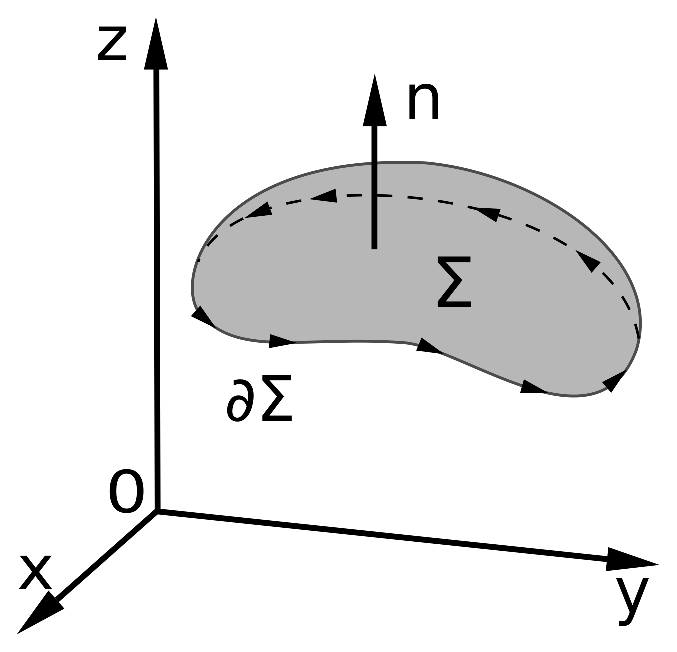
\includegraphics[width=0.7\linewidth]{Immagini/stokes.eps}
        \caption{Here we divide the surface of the sphere in two different surfaces $\mathcal A$ and $\mathcal B$ that share the edge $\mathcal P$}
    \end{figure}
    From the Stokes theorem we have that
    \begin{equation}
        \label{eq:stokes}
            \gamma_n=\oint_\mathcal{P} A^n_\mu\: d\lambda^\mu=\frac 12 \int_\Sigma \Omega_{\mu\nu}^n\: d\lambda^\mu \wedge d\lambda^\nu\,,
    \end{equation}
    where we have used the Einstein convention of summation.\newline
    There is a subtelty in this last equation, as we know the Berry curvature tensor in Gauge-invariant, so the integral over the surface is too, but the integral over the closed path of the Berry connection is defined up to a factor $2n\pi$ that is gauge dependant.
    So is there a modulo $2\pi$ ambiguity or not?\newline
    The answer is that if $\gamma_n$ is to be determined using the knowledge of $\ket{n,\boldsymbol \lambda}$ 
    only on the curve $\mathcal P$ then it is really well defined modulo $2\pi$. In this case we can re-write 
    equation \ref{eq:stokes} as 
    \begin{equation}
    \frac 12 \int_\Sigma \Omega_{\mu\nu}^n\: d\lambda^\mu \wedge d\lambda^\nu:=\oint_\mathcal{P} A^n_\mu\: d\lambda^\mu\,.
    \end{equation}
    Meaning that the integral over the surface $\Sigma$ is equal to \textit{one of the values of} the integrals along the closed path $\mathcal P$.

    But what kind of Gauge gives the "correct" answer? If we choose a gauge that is continuous and smooth
    everywhere along the surface $\Sigma$ including on its boundary $\mathcal P$ then equation \ref{eq:stokes} becomes unambiguous.\newline
    While it is possible to make a radical gauge transformation that shifts $\gamma_n$ by $2\pi$ when regarding $\ket{n,\boldsymbol \lambda}$ as a function defined only in the neighborhood of $\mathcal P$, such a gauge change cannot be smoothly continued into the interior $\mathcal S$ without creating a vortex-like singularity of $\gamma_n(\boldsymbol \lambda)$.


\section{Chern Theorem}
    
    Let's take as an example Gauss's theorem. It tells us that the flux of the field through a closed surface is equal to the charges inside. \newline
    Now let's calculate the flux of the Berry curvature through a closed surface. We can divide the closed surface as two different open surfaces that share the same edge $\mathcal P$.\newline
    Thanks to stokes theorem the flux through the surface $\mathcal A$ is $\oint_\mathcal{P} \mathbf A \cdot d\boldsymbol \lambda$, but the flux through the surface $\mathcal B$ is $-\oint_\mathcal{P} \mathbf A \cdot d\boldsymbol \lambda$.\newline
    Theese two integrals must be equal modulo $2\pi$, so
    \begin{figure}
        \centering
        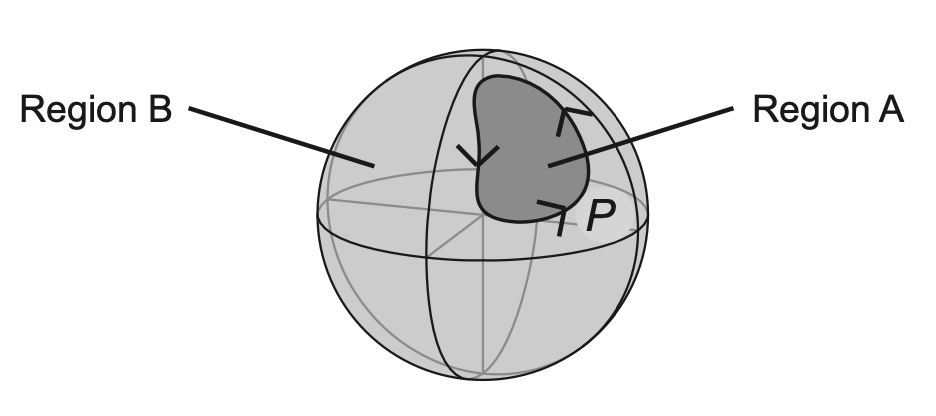
\includegraphics[width=0.85\linewidth]{Immagini/topo/chern_theorem.png}
        \caption{Here we divide the surface of the sphere in two different surfaces $\mathcal A$ and $\mathcal B$ that share the edge $\mathcal P$}
        \label{fig:forward_pass}
    \end{figure}
    \begin{equation}
        \label{eq:chern}
        \oint_\mathcal{S} \Omega_{\mu\nu}^n d\lambda^\mu \wedge d\lambda^\nu =2\pi C_n \quad\quad C_n\in \mathbb Z\,.
    \end{equation}
    This means that the flux thought a closed surface of the Berry curvature is quantized
    
    The constant $C$ in known as the Chern number. Note that when the Chern index is nonzero, it is impossible to construct a smooth and continuous gauge over the entire surface $\mathcal{S}$. If such a gauge did exist, then we could apply Stokes’ theorem directly to the entire surface and conclude that the Chern number vanishes, in contradiction with the assumption.\newline
    But what are these "pseudo-charges" inside the closed surface that generate the flux?\newline
    In E.M. a simple way to spot charges (or monopoles) is to look at the fields and see if as some point it diverges as $1/(\mathbf r-\mathbf{r_0})^2$. Let's take a look at $\Omega_{\mu\nu}$ (eq. \ref{eq:berry-curvature3}) and see if we can spot anything similar \footnote{In the equation below I expressed explicitly the $\boldsymbol \lambda$ dependence in the denominator and condensed the formula using the wedge product $\wedge$}
    \begin{equation}
        \label{eq:monopoles1}
        \Omega_{\mu\nu}^n=i\sum_{n'\neq n} \frac{\bra{n}\partial_\mu H\ket{n'}\wedge \bra{n'} \partial_\nu H\ket{n}}
        {\underbrace{[E_{n'}(\boldsymbol \lambda)-E_n(\boldsymbol \lambda)]^2}_
        {\substack{\text{what happens if for some } \boldsymbol \lambda=\boldsymbol \lambda_d  \\\text{ the two energies are the same?}}}}\,.
    \end{equation}
    So, suppose that for some $\boldsymbol \lambda=\boldsymbol \lambda_d$ we have that $E_n (\boldsymbol \lambda_d)=E_m(\boldsymbol \lambda_d)$, now we expand the energies near $\boldsymbol \lambda_d$ at first order
    \[
    \begin{cases}
    E_n(\boldsymbol \lambda)\, \approx E_n(\boldsymbol \lambda_d) +\, \partial_{\boldsymbol \lambda} E_n|_{\boldsymbol \lambda =\boldsymbol \lambda_d}\cdot (\boldsymbol \lambda-\boldsymbol \lambda_d)\\
    E_m(\boldsymbol \lambda)\approx E_n(\boldsymbol \lambda_d) + \partial_{\boldsymbol \lambda} E_m|_{\boldsymbol \lambda =\boldsymbol \lambda_d}\cdot (\boldsymbol \lambda-\boldsymbol \lambda_d)\\

    \end{cases}\,.
    \]
    This means that 
    \[
    E_n(\boldsymbol \lambda)-E_m(\boldsymbol \lambda)\approx \partial_{\boldsymbol \lambda} (E_n-E_m)|_{\boldsymbol \lambda =\boldsymbol \lambda_d}\cdot (\boldsymbol \lambda-\boldsymbol \lambda_d)\,,
    \]
    so the denominator of the berry curvature near $\boldsymbol \lambda_d$ goes like $ 1/(\boldsymbol \lambda-\boldsymbol \lambda_d)^2$.\newline
    This means that there are "charges" or "monopoles" that induce the flux through the closed surface, and they are localized where 2 (or more) energy levels cross


	
	
	
	\printbibliography

\end{document}